\documentclass[fleqn,10pt]{SelfArx} % Document font size and equations flushed left

\usepackage[english]{babel} % Specify a different language here - english by default
\setlength{\columnsep}{0.55cm} % Distance between the two columns of text
\setlength{\fboxrule}{0.75pt} % Width of the border around the abstract
\definecolor{color1}{RGB}{0,50,100} % Color of the article title and sections
\definecolor{color2}{RGB}{0,20,20} % Color of the boxes behind the abstract and headings
\usepackage{hyperref} % Required for hyperlinks
\hypersetup{
	hidelinks,
	colorlinks,
	breaklinks=true,
	urlcolor=color2,
	citecolor=color1,
	linkcolor=color1,
	bookmarksopen=false,
	pdftitle={Title},
	pdfauthor={Author},
}
\JournalInfo{10th May, 2024} % Journal information
\Archive{Math 399 Independent Study Final Project} % Additional notes (e.g. copyright, DOI, review/research article)

\PaperTitle{Performance-Based Clustering and Classification Analysis of NBA Players} % Article title

\Authors{Qisong(Andrew) Gou\textsuperscript{1}, Shuorui(Ray) Li\textsuperscript{2}} % Authors
\affiliation{\textsuperscript{1}\textit{Hamilton College, Clinton, NY, United States}} % Author affiliation
\affiliation{\textsuperscript{2}\textit{Hamilton College, Clinton, NY, United States}} % Author affiliation

\Keywords{NBA --- Classification --- Principal Component Analysis --- K-means clustering --- Random Forest} % Keywords - if you don't want any simply remove all the text between the curly brackets
\newcommand{\keywordname}{Keywords} % Defines the keywords heading name

\Abstract{This study employs a combination of statistical methods to classify NBA players based on their performance during the 2021-2022 season. Principal Component Analysis (PCA) is used to reduce the dimensionality of the dataset while retaining the most significant features that explain the variance in player statistics. K-means clustering is then applied to the transformed dataset to partition players into distinct clusters based on their proximity to the centroid of each cluster. The optimal number of clusters is determined using the elbow method. The analysis identifies four distinct player clusters: The Consistent Role Players, The Developing Perimeter Players, The All-Stars, and The Supportive Contributors. A Random Forest model is built to explore the importance of variables and provide insights into the key performance indicators that differentiate player clusters. The model also highlights Offensive Rebounds, Field Goals, Blocks, and Points as the most influential features in predicting player performance. The study offers insights into modern basketball team-building trends and the characteristics of successful player archetypes.}

%----------------------------------------------------------------------------------------

\begin{document}

\maketitle % Output the title and abstract box

\tableofcontents % Output the contents section

\thispagestyle{empty} % Removes page numbering from the first page

\section*{Introduction} % The \section*{} command stops section numbering

\addcontentsline{toc}{section}{Introduction} % Adds this section to the table of contents
Basketball is a dynamic team sport that involves two teams of five players each, competing on a rectangular court to score points by shooting a ball through a hoop. The sport was invented by Dr. James Naismith in 1891 to offer a safer sport to football, the game has since evolved into a global phenomenon enjoyed by millions in amateur and professional settings.\\
The National Basketball Association (NBA) is the premier professional basketball league in the world, founded in 1946 as the Basketball Association of America (BAA) before adopting its current name in 1949 following a merger with the National Basketball League (NBL). The NBA consists of 30 teams, divided into the Eastern and Western Conferences. Known for its high level of competition and entertainment, the NBA has helped popularize basketball worldwide, making household names of its top players and contributing significantly to the sport's global appeal. The NBA season is divided into the regular season and the playoffs, featuring intense competition and showcasing the athletic prowess of its players.\\
During the regular season, each of 30 teams plays 82 games, split evenly between home and away matchups. This format is designed to determine standings, with teams vying for a favorable position in order to qualify for the playoffs. Following the regular season, the top eight teams from each conference advance to the playoffs, a high-stakes elimination tournament that ultimately decides the NBA champion.  Each playoff encounter between two distinct teams is a series of seven games. The team that first wins four games advances to the next round. The intensity of the playoffs often brings out the best in players, with careers defined and legacies formed during critical games. The culmination of the playoffs is the NBA Finals, where the champions of the Eastern and Western Conferences face off in a final best-of-seven series to determine the league champion, an event that attracts a global audience and highlights the pinnacle of professional basketball competition.\footnote{The official site of the NBA for the latest NBA Scores, Stats \& News. $|$ NBA.com, http://nba.com. Accessed 10 May 2024.}\\
Over the years, team building in the NBA has evolved significantly, adapting to changes in player dynamics, league rules, and technological advancements. Traditionally, teams focused on acquiring balanced rosters through drafts and trades, emphasizing a mix of scoring, defense, and leadership. The 1980s and 1990s saw teams built around dominant centers and all-around superstars, aiming for a blend of youth and veteran presence. However, the 2000s ushered in the "Big Three" era, where franchises sought to assemble trios of superstar talents to compete for championships, a trend popularized by the Boston Celtics and Miami Heat. More recently, the focus has shifted towards versatility and space creation, emphasizing three-point shooting and high-paced offense. Advanced analytics now play a crucial role in player evaluations and game strategies, leading teams to prioritize efficiency and adaptability in their roster constructions. This shift reflects a broader trend of data-driven decision making in sports. With advancements in data science and technology, teams can now access an increasingly high amount of player data. Machine learning allows teams to place a specific player within a distinct cluster based on performance related statistics. \\
This study employs a combination of statistical methods to classify NBA players based on their performance during the 2021-2022 season. The primary goal of this research is to use Principal Component Analysis and K-means clustering to statistically group players into clusters reflective of their skills and performance, and build a Random Forest model to explore the importance of variables, make predictions, and potentially reveal the crucial attributes for each player. The characteristics of new clusters will be analyzed and interpreted to offer some insights on modern basketball team-building trends and how to build a good team. 



%------------------------------------------------

\section*{Materials}
\addcontentsline{toc}{section}{Materials}
The data for this study is sourced from Basketball Reference's open-access website (http://www.basketball-reference.com/), providing individual performance statistics for NBA players during the 2021-2022 season. By focusing on the most recently completed season on the website, the analysis incorporates contemporary strategies and player performances, ensuring its relevance to current and future trends in the NBA. This approach enhances the applicability and timeliness of the study's findings, allowing for insights that can inform decision-making within the rapidly evolving landscape of professional basketball.\\
The initial dataset included an extensive array of performance metrics for each player. To prepare the data for analysis, a series of pre-processing steps were undertaken.\\First, the repeated and redundant data for the same players in the same season were removed. For players who served in more than one team in one season, only the metrics of first team were kept.\\Second,
to ensure the relevance of the analysis, the data was filtered to include only records from the 2021-2022 season. Additionally, missing values were addressed by imputing zeros, particularly in percentage metrics. This imputation was based on the assumption that missing values in shooting categories indicated no attempts made by the player, thus reflecting no activity in those specific areas. \\Third, irrelevant columns such as extra identifiers were removed to focus the dataset on quantitative metrics. \\Finally,the columns that can be directly computed from other columns such as Three-Point Percentage (3P\% = 3P/3PA) and Two-Point Percentage (2P\% = 2P/2PA) were removed to reduce the dependence among variables.\\
The dataset encompasses a broad spectrum of metrics (as shown in Table 1), including Games (G), Games Started (GS), Minutes Played Per Game (MP), Points Per Game (PTS), Field Goals Per Game (FG), Field Goal Attempts Per Game (FGA), Effective Field Goal Percentage (eFG\%), 3-Point Field Goals Per Game (3P), 3-Point Field Goal Attempts Per Game (3PA), 2-Point Field Goals Per Game (2P), 2-Point Field Goal Attempts Per Game (2PA), Free Throws Per Game (FT), Free Throw Attempts Per Game (FTA), Offensive Rebounds Per Game (ORB), Defensive Rebounds Per Game (DRB), Assists Per Game (AST), Steals Per Game (STL), Blocks Per Game (BLK), Turnovers Per Game (TOV), Personal Fouls Per Game (PF). These metrics provide a comprehensive overview of player performance, capturing aspects of scoring efficiency, defensive contributions, and overall impact on the game. 
\begin{figure}[ht]
    \centering
    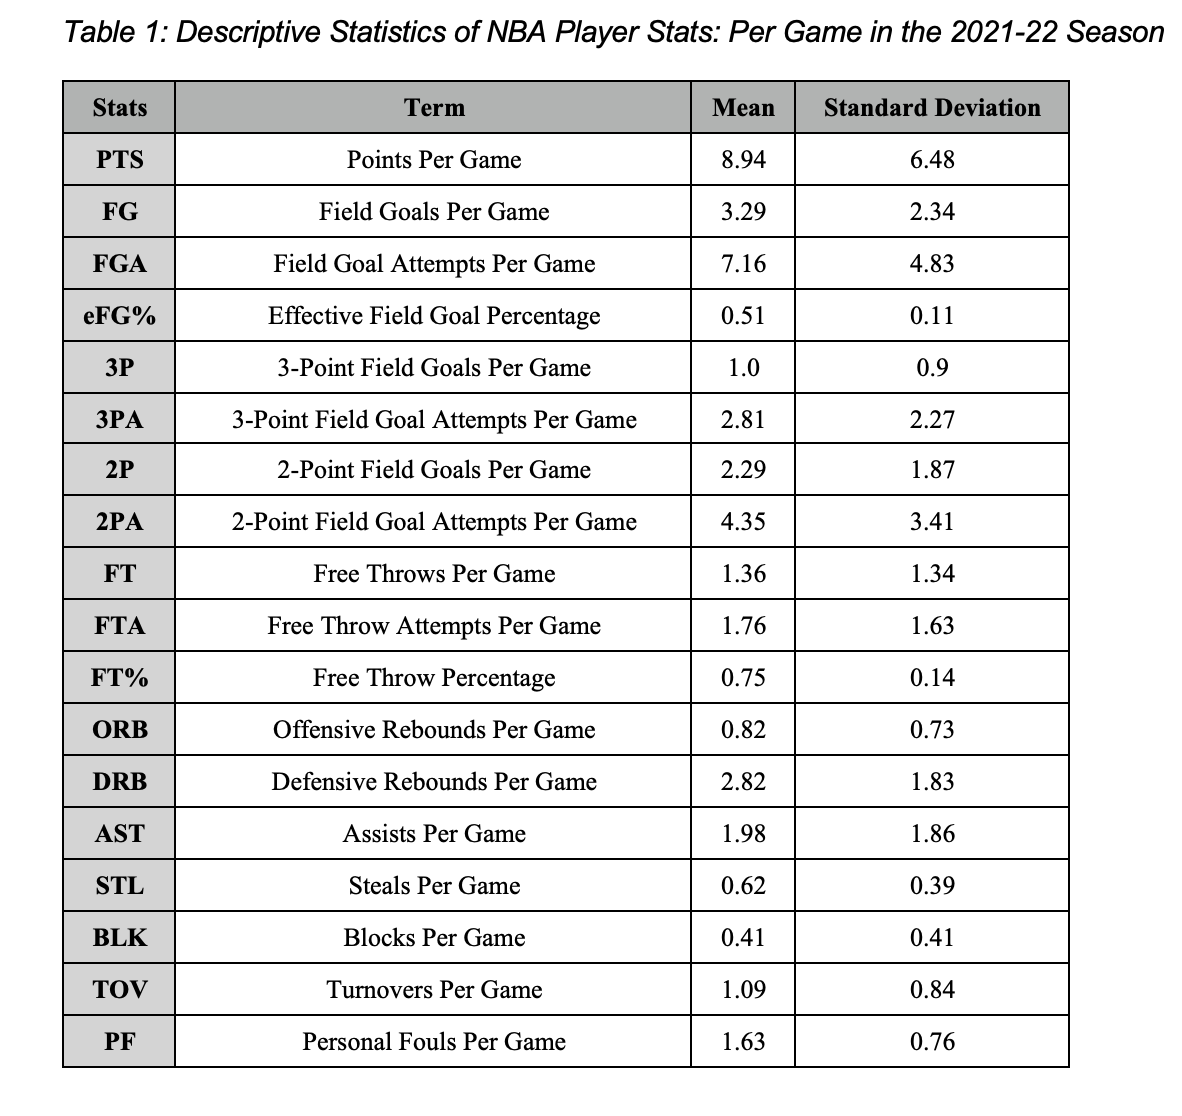
\includegraphics[width=\linewidth]{Figure/table1.png}
\end{figure}

\section*{Principal Component Analysis}
\addcontentsline{toc}{section}{Principal Component Analysis}
Principal Component Analysis (PCA) is utilized as the first step in our analysis to reduce the dimensionality of the dataset. This technique transforms the original variables into a new set of variables -  linear combinations of the original variables. These new variables, called principal components, are orthogonal and ranked according to the variance they capture from data. For this study, components that contribute significantly to the variance were retained, ensuring that the most relevant features for player performance are preserved while reducing computational complexity and eliminating multicollinearity.
\begin{figure}[ht]
\centering
\centering
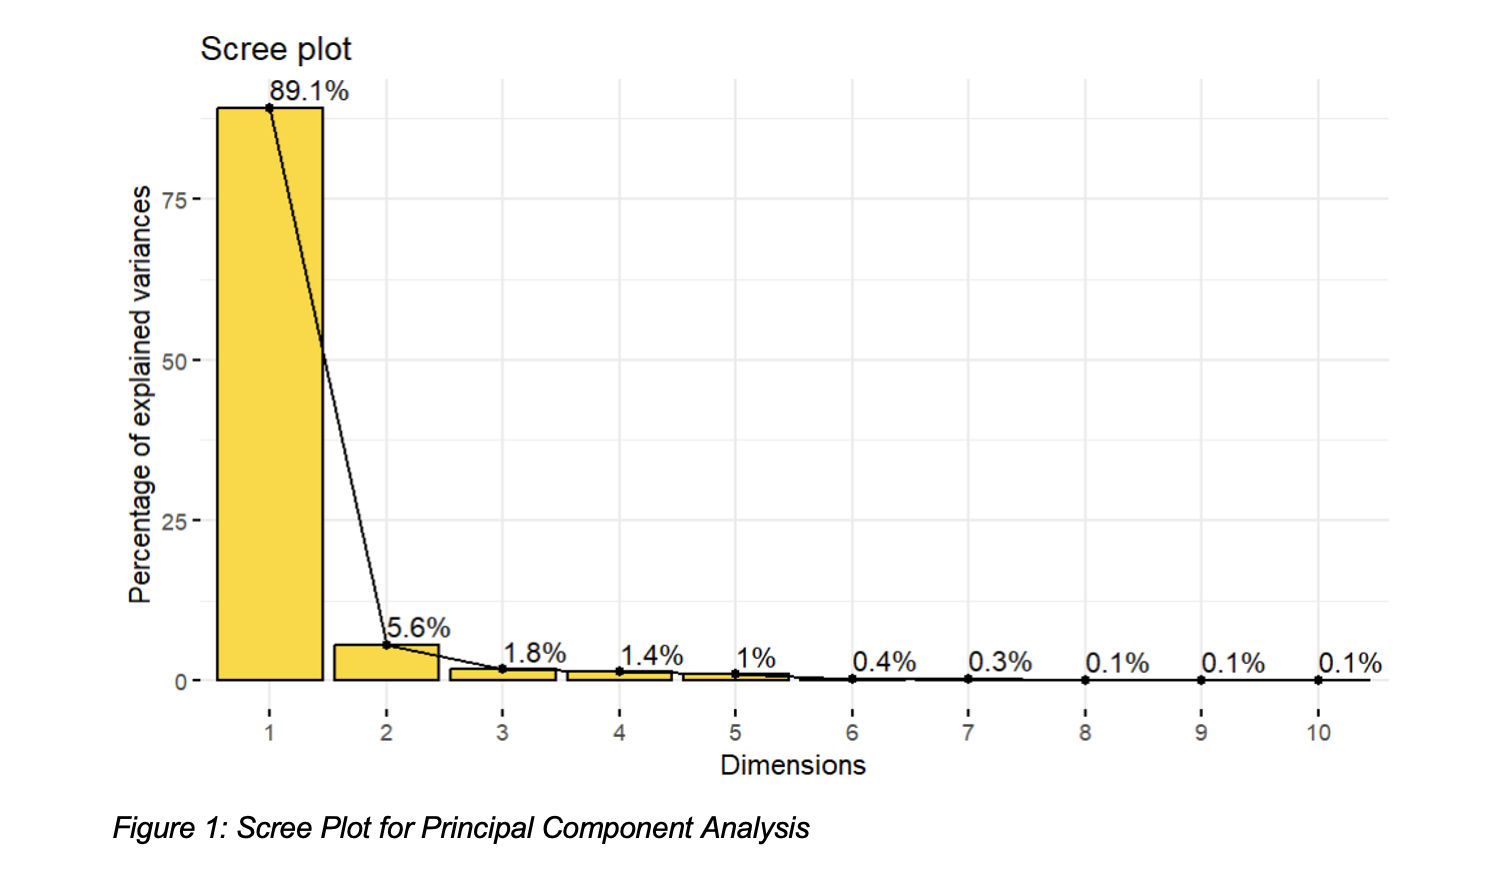
\includegraphics[width = \linewidth]{Figure/figure1.png}
\end{figure}
\\The primary goal of using PCA was to reduce the dimensionality of the 2021-2022 NBA player statistics dataset while retaining the most significant features that explain the variance in our dataset. The dataset was standardized to ensure that each feature contributed equally to the analysis, given the different scales of the original variables. PCA was then applied to the standardized features.\\
Figure 1 shows the percentage of variance explained by the number of principal components. The proportion of variance explained by the principal components increases with the number of components, providing guidance in determining the optimal number of components required to capture a substantial portion of the information present in the data. The first two components were chosen because they already capture about 94\% of the variance and choosing two components makes it easier to visualize player data and interpret player clusters in the following sections.
\\
The PCA Plot (Figure 3) and the Variable Loadings Chart (Table 2) reveal more valuable information. Specifically, Principal Component 1 is strongly influenced by variables including Points (PTS) with a loading of 0.66590819, Field Goal Attempts (FGA) with 0.49352938, and is moderately influenced by 2-Point Attempts (2PA) with a weight 0.33070254, Field Goals (FG) with 0.24069096 and  3-Point Attempts (3PA) with 0.16282889. Component 1 primarily captures scoring ability, emphasizing direct point contributions (PTS) and shot attempts (FGA). This component appears to focus on players who are actively involved in offensive plays, taking many shots, particularly field goals and 2-point shots. Thus, this component could be viewed as a "scoring and shooting activity" factor, representing players who are central to the offensive strategy. \\
Principal Component 2 is strongly influenced by variables such as 3-Point Attempts (3PA) with a loading of 0.657668284, and moderately influenced by 3-Points (3P) with 0.262021633, Field Goal Attempts (FGA) with 0.207617661. Also, PC 2 is negatively influenced by 2-Point Attempts (2PA) and 2-Points (2P) with loadings of -0.450052752 and -0.299384391 respectively, and Defensive Rebounds (DRB) with -0.256743255. Component 2 seems to capture specialization in long-range shooting, particularly focusing on players who attempt and likely make a significant number of 3-point shots. The negative loadings on 2-point attempts and defensive contributions suggest a contrast between players who specialize in perimeter play versus those involved in more traditional inside roles or defensive efforts. This component might be considered as a "perimeter specialization" factor, emphasizing players' roles as 3-point shooters who might not be as involved in inside play or defense.\\
Overall, Component 1 identifies primary scorers who take a high volume of shots, especially from inside the arc, highlighting their role in driving the offensive play, while Component 2 differentiates players based on their specialization in 3-point shooting, distinguishing those who contribute significantly from beyond the arc, which is increasingly valuable in modern basketball strategies.\\
\begin{figure}[ht]
    \centering
    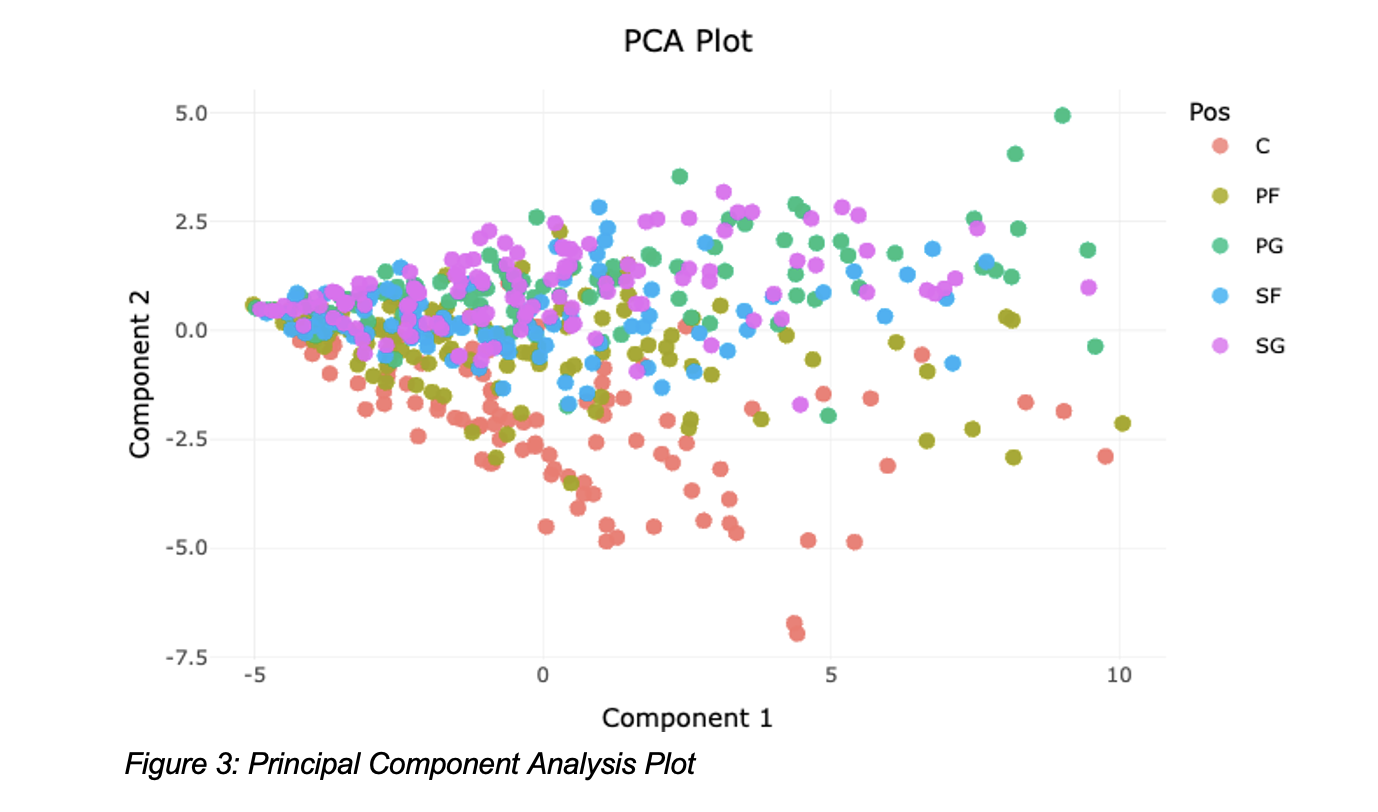
\includegraphics[width = \linewidth]{Figure/figure3.png}
    \label{fig:enter-label}
\end{figure}
\begin{figure}[ht]
    \centering
    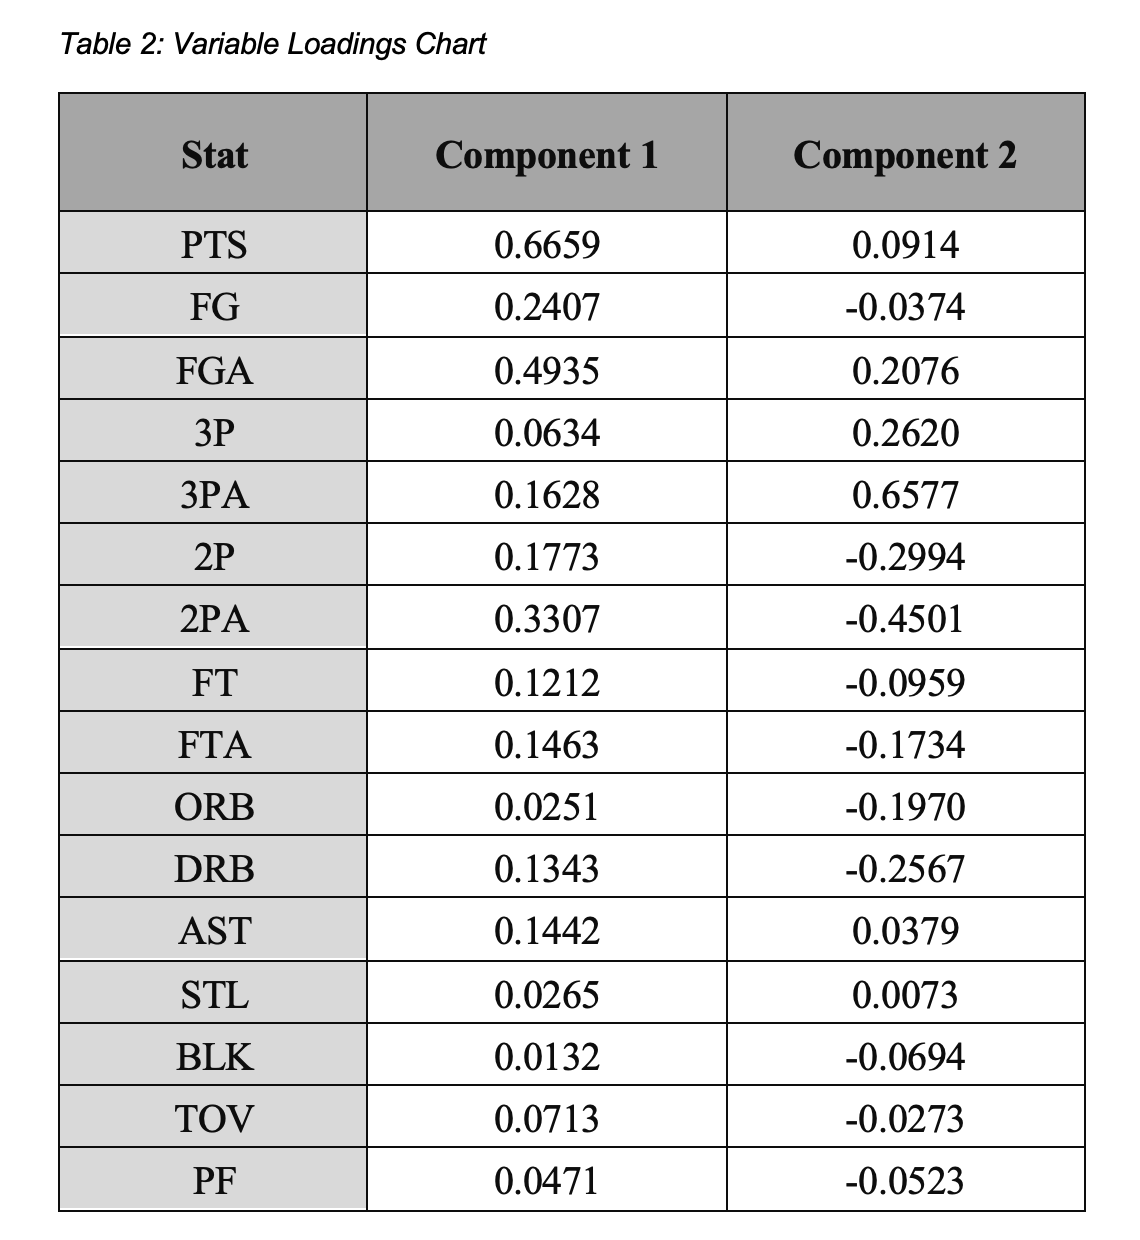
\includegraphics[width = \linewidth]{Figure/table2.png}
    \label{fig:enter-label}
\end{figure}

\section*{K-Means Clustering}
\addcontentsline{toc}{section}{K-Means Clustering}
\begin{figure*}[ht]
    \centering
    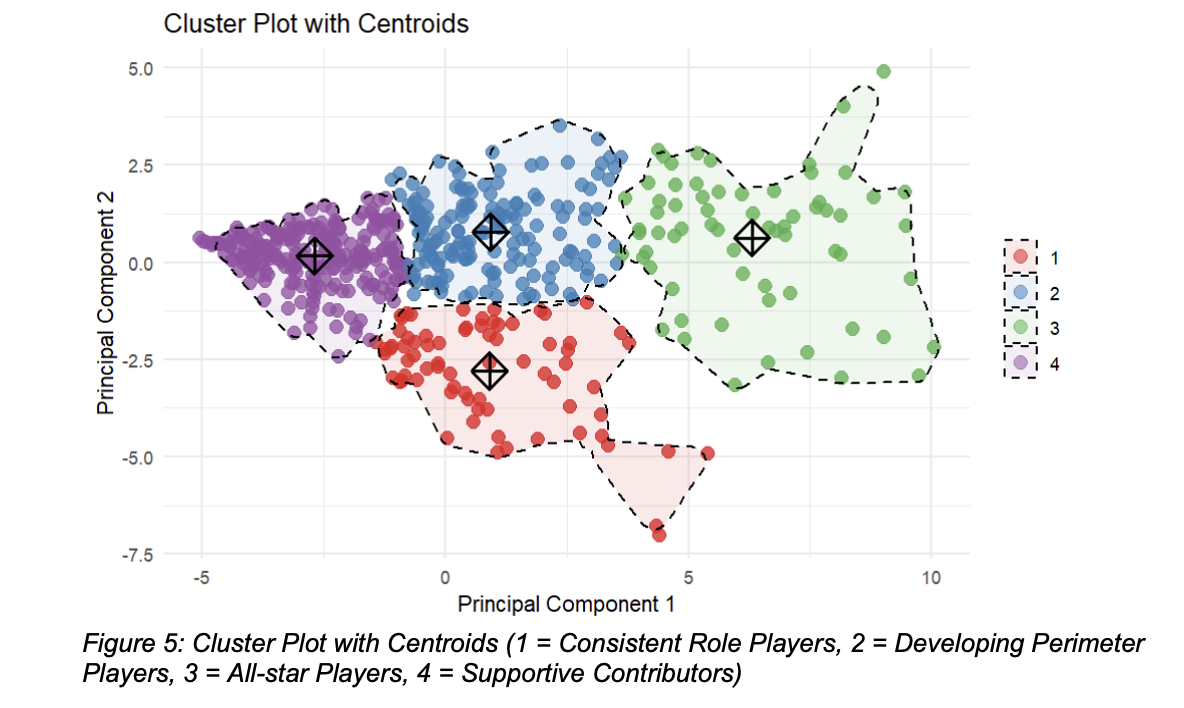
\includegraphics[width = 0.8\linewidth]{Figure/figure5.png}
    \label{fig:enter-label}
\end{figure*}
Following dimensionality reduction, K-means clustering is applied to the transformed dataset. This algorithm partitions the players into clusters based on their proximity to the centroid of the clusters to minimize the within-cluster sum of squares. The optimal number of clusters is determined using the elbow method (see Figure 4), which involves plotting the sum of squared distances from each point to its assigned center and choosing the kink point as the appropriate number of clusters.\\
The elbow method plot displays the sum of squared distances for each number of clusters $(k)$ from 1 to 10. The "elbow" point in the graph is typically used to choose the optimal number of clusters, which is where the rate of decrease sharply shifts, indicating diminishing returns by adding more clusters. In this plot, there seems to be an elbow around $k = 4$, suggesting that four clusters might be a reasonable choice for grouping the players.\\
\begin{figure}[ht]
    \centering
    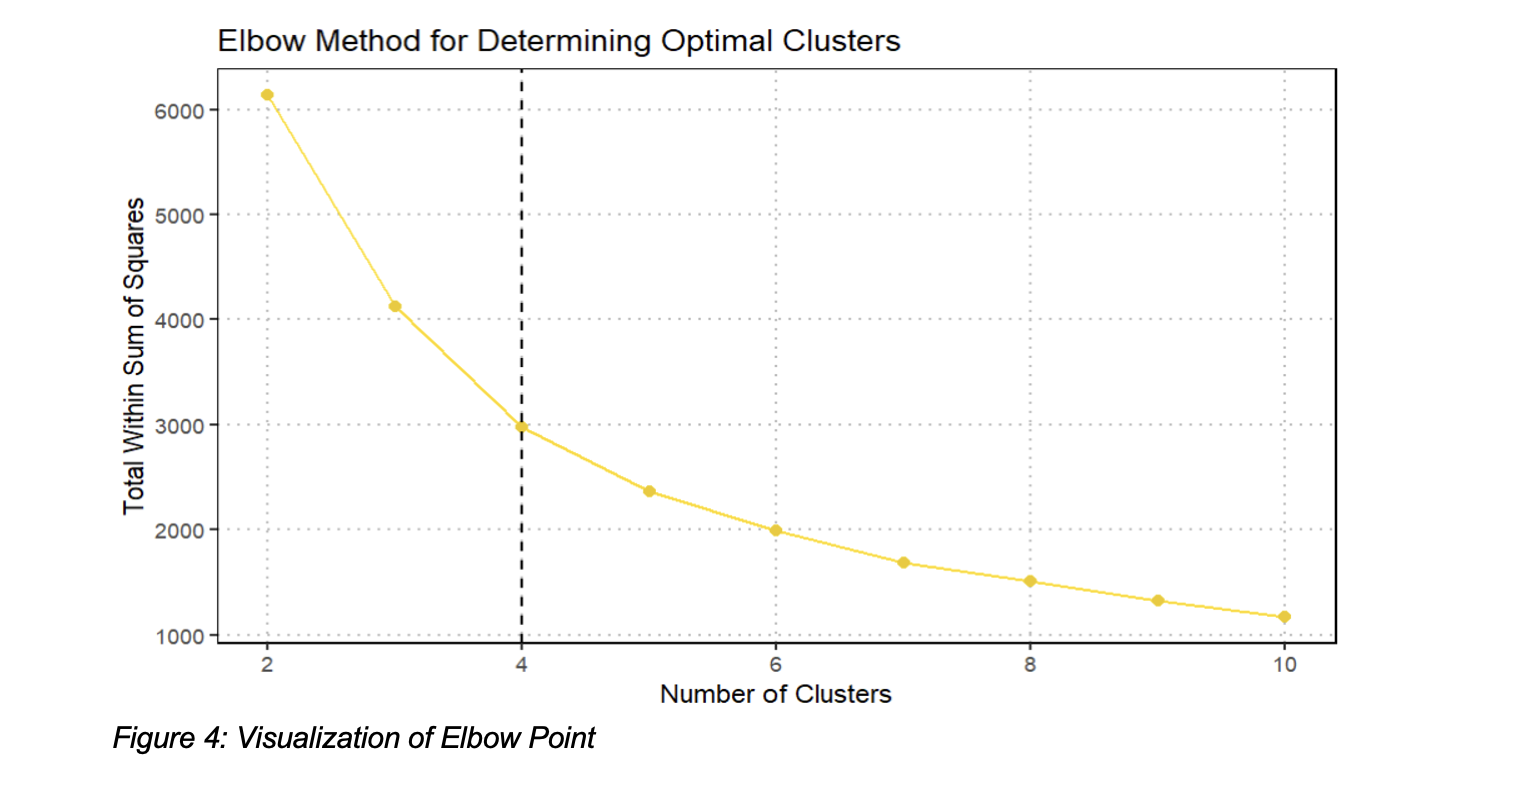
\includegraphics[width = \linewidth]{Figure/figure4.png}
    \label{fig:enter-label}
\end{figure}\\
Figure 5 demonstrates the the application of K-means clustering method to the NBA player statistics from the 2021-2022 season, based on the previous results of two principal components PC1 and PC2. This plot shows how players, with similar performance and statistical profiles, are grouped into the same cluster. In total, there are four different clusters being created using the centroid method (as shown in Figure 5 and Table 3): \\
\begin{figure}[ht]
    \centering
    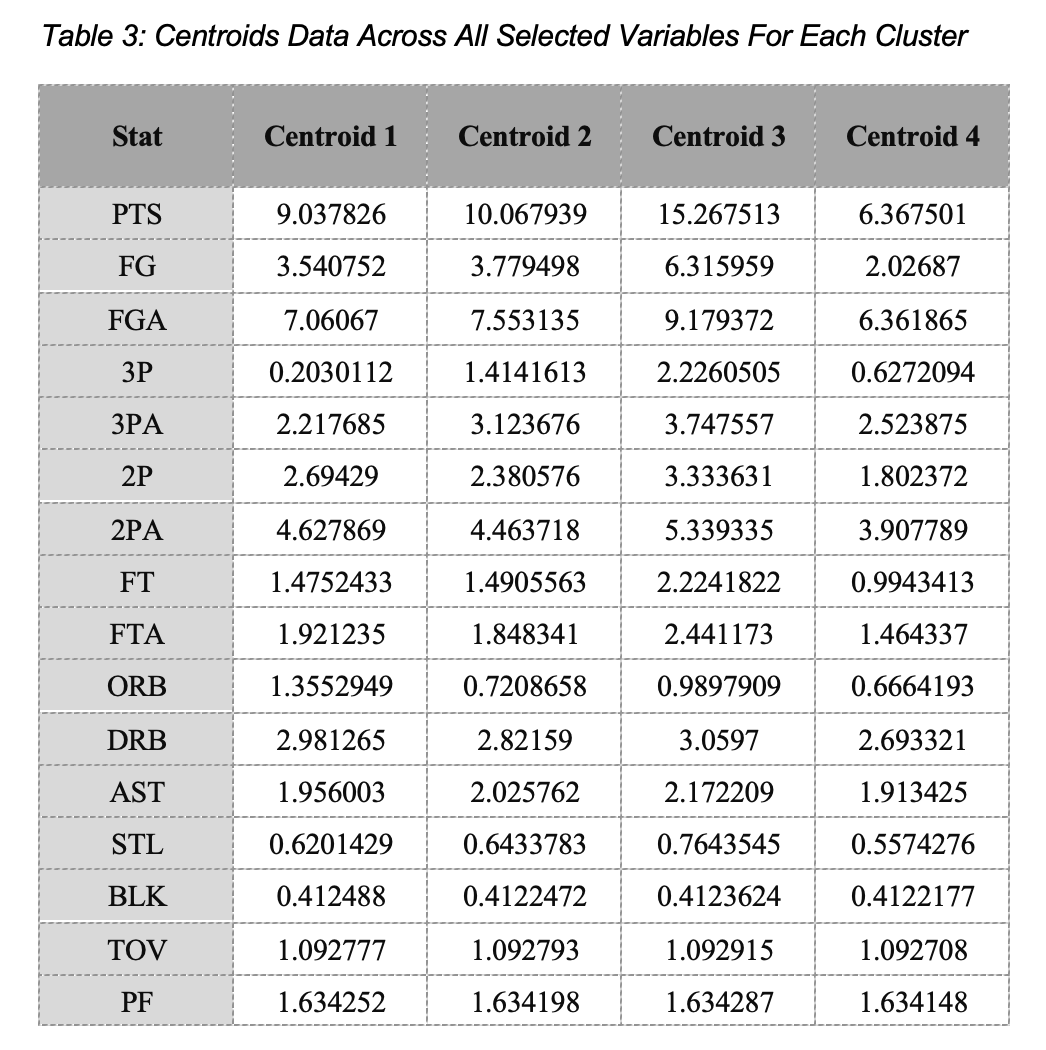
\includegraphics[width = \linewidth]{Figure/table3.png}
    \label{fig:enter-label}
\end{figure}\\
\textbf{Cluster 1 --- The Consistent Role Players}: Players in this cluster score moderately with an average of 9.04 points and have a decent shooting efficiency with 3.54 field goals made out of 7.06 attempts. They show a lower frequency in three-point shooting, suggesting their play is more oriented towards inside scoring. These players likely fill specific roles such as secondary scorers or key defensive players, providing consistent contributions but not serving as the primary offensive option. Their moderate rebound and assist numbers support their involvement in various facets of the game, making them reliable but not standout performers.\\
\textbf{Cluster 2 --- The Developing Perimeter Players}: This cluster includes players who are slightly more prolific scorers with an average of 10.07 points. They are significantly involved in perimeter shooting, averaging 1.41 three-pointers out of 3.12 attempts. These stats suggest that these players are evolving into significant contributors, particularly in strategies that emphasize spacing and outside shooting. They might be transitioning into more central roles within their teams, supported by their ability to stretch defenses and contribute effectively from beyond the arc.	\\
\textbf{Cluster 3 --- The All-Stars}: Featuring the highest averages in points (15.27), field goals made (6.32), and three-point shots (2.23), players in this cluster are the primary offensive options for their teams. Their high assists and shot attempts indicate their centrality in offensive plays and their ability to score from both inside and outside the arc. These players are versatile and pivotal, often taking on multiple responsibilities including scoring, playmaking, and leadership, which makes them the stars and key performers in crucial game situations.\\
\textbf{Cluster 4 --- The Supportive Contributors}: The players in this cluster are characterized by the lowest scoring average at 6.37 points, but they still attempt a reasonable number of shots, including 2.52 three-point attempts. They are likely not the primary scoring options but are valued for their ability to fill various roles, possibly including specific defensive tasks or situational plays. Their contribution is essential for maintaining team dynamics and executing game plans, making them critical, albeit less highlighted, members of their teams.
%------------------------------------------------
\section*{Random Forest}
\addcontentsline{toc}{section}{Random Forest}
Using the entire dataset with cluster assignments from K-means results as labels and a 50-50 training and testing split to build a Random Forest model which leverages a robust ensemble learning method to predict NBA player performance, it is interested to see how well the model can make the prediction on which cluster a player belongs to, given his various attributes and on-court performances.
\begin{figure}[ht]
    \centering
    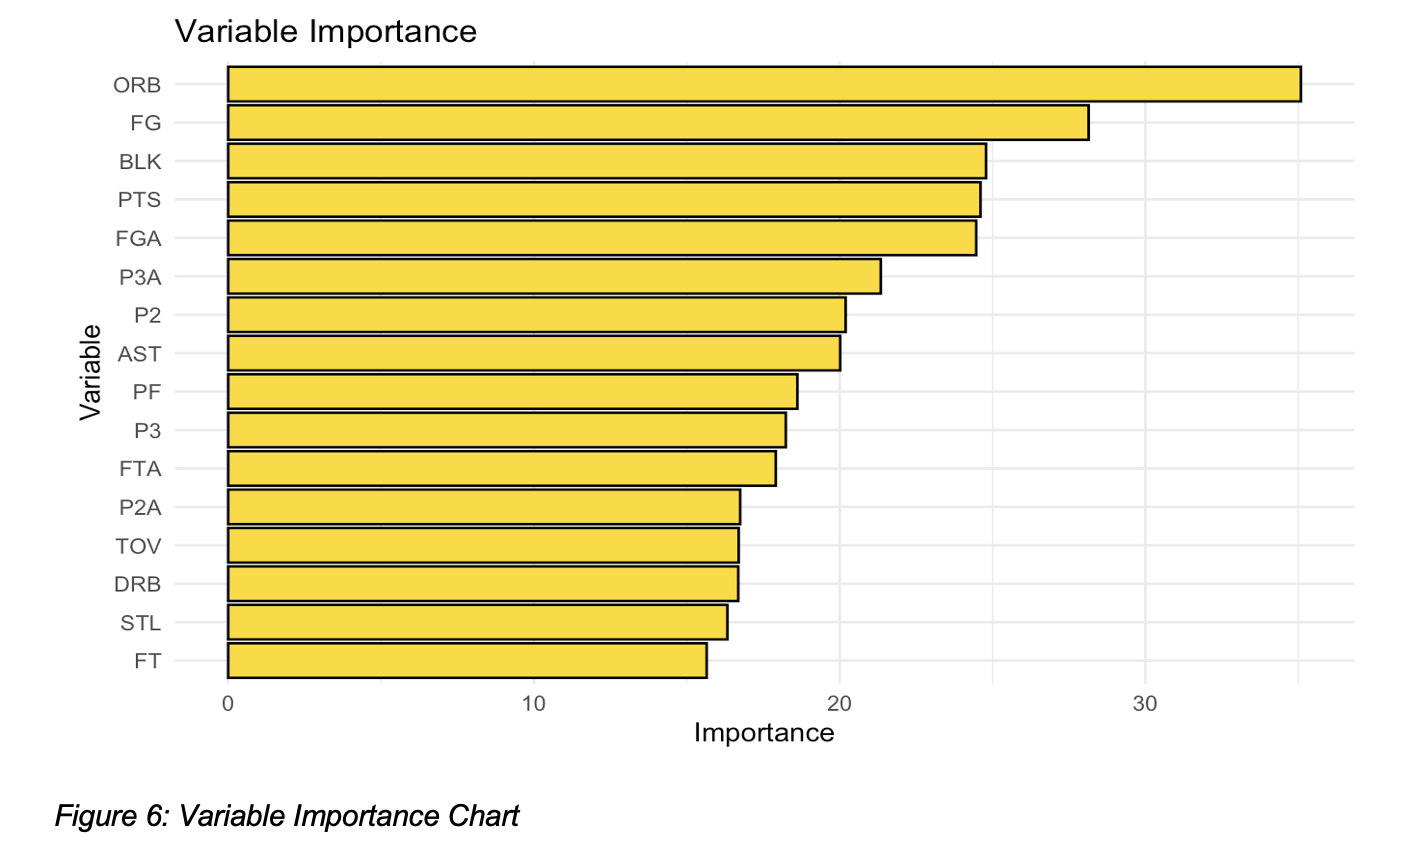
\includegraphics[width = \linewidth]{Figure/figure6.png}
    \label{fig:enter-label}
\end{figure}
\\The variable importance graph (Figure 6) offers several key insights, identifying Offensive Rebounds (ORB), Field Goals (FG), Blocks (BLK), and Points (PTS) as the most influential features in determining a player's impact and effectiveness during games. For instance, the prioritization of ORB suggests a strong correlation between securing offensive rebounds and subsequent scoring opportunities or game control, thereby establishing it as a potent predictor of player value.
\begin{figure}[ht]
    \centering
    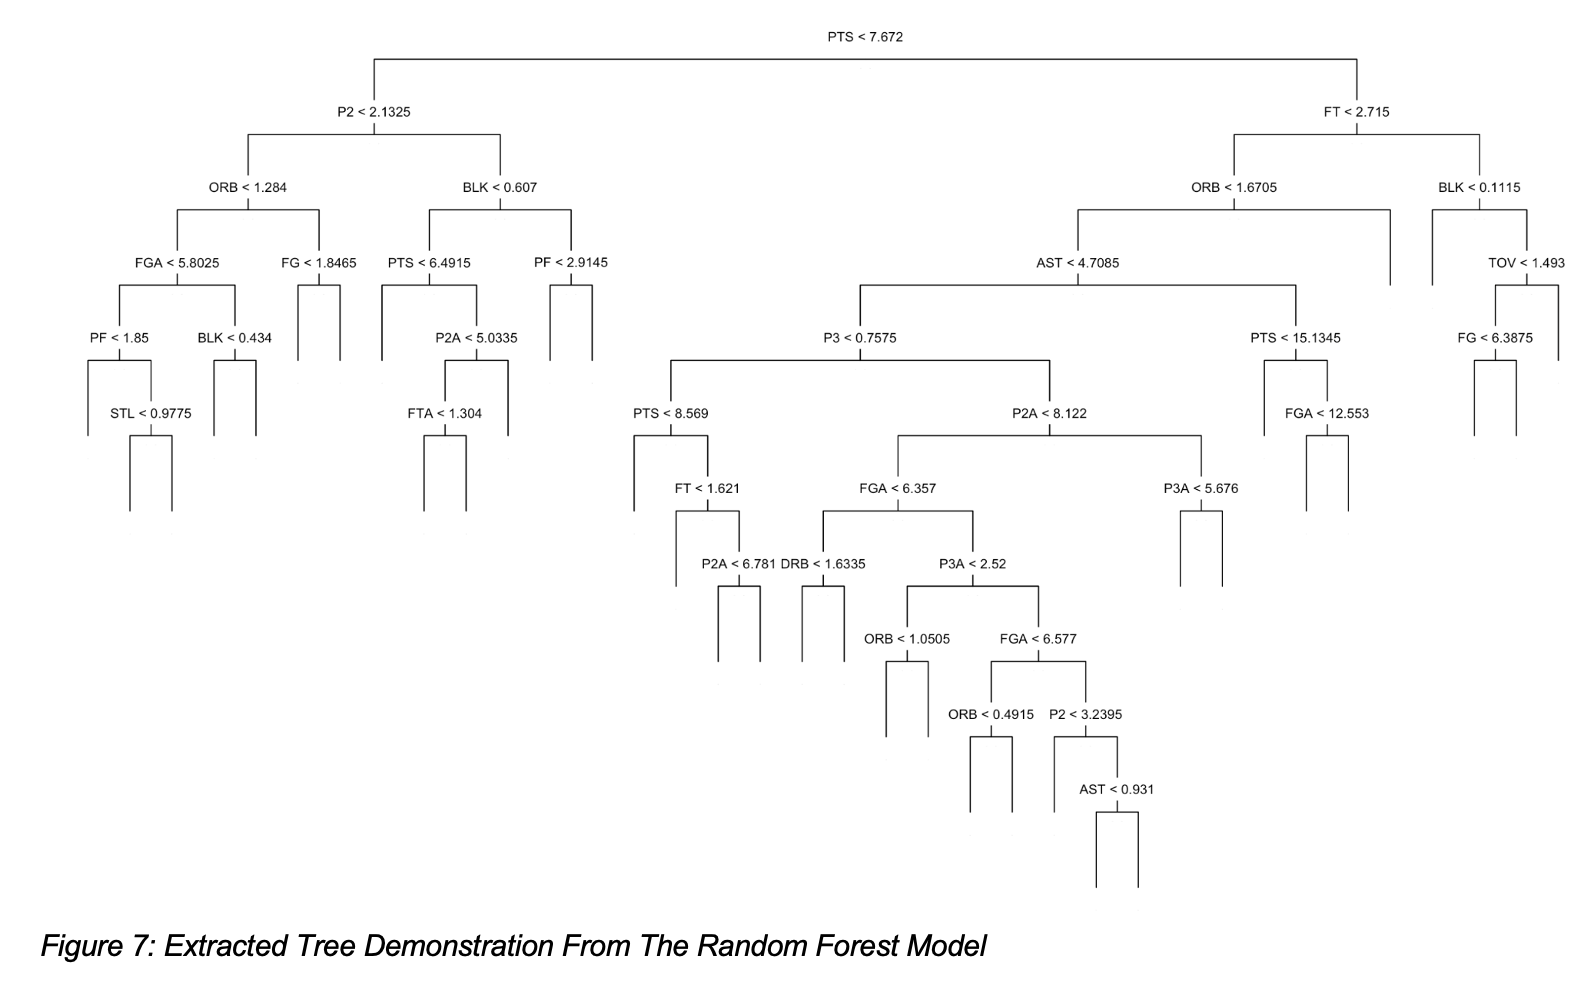
\includegraphics[width = \linewidth]{Figure/figure7.png}
    \label{fig:enter-label}
\end{figure}
\\This importance is further exemplified in the decision tree (Figure 7) extracted from the Random Forest model, which reveals the intricate manner in which individual trees navigate the dataset to arrive at a prediction. The tree commences by assessing a player's scoring ability through PTS thresholds, distinguishing between low-scoring and higher-scoring players. As the tree progresses, more nuanced splits emerge, such as ORB $<$ 1.284 or BLK $<$ 0.607, pinpointing the significance of specific plays that often lead to changes in possession or scoring opportunities, reflecting a player's defensive prowess and ability to maintain or shift game momentum.\\
Furthermore, the tree evaluates field goals made (FG) and attempted (FGA), illustrating a player's shooting efficiency and decision-making in shot selection. Thresholds like P2A $\leq$ 5.0335 and P3A $<$ 2.52 highlight an analytical dive into a player's shooting range and preferences, informing strategies on player utilization or defensive setups. The tree's branches also consider turnovers (TOV) and fouls (PF), addressing a player's game discipline and risk-taking behavior.\\
By capturing these complex patterns and interactions among multiple features, the Random Forest model provides a multidimensional analysis of player performance, turning raw statistical data into actionable insights. Moreover, the model shows its strong ability to integrate these insights into an ensemble prediction that reduces variance and avoids overfitting, as evidenced by the error rate graph (Figure 8), which shows a robust decline in error rates with an increase in the number of trees, stabilizing after approximately 100 trees.
\begin{figure}[ht]
    \centering
    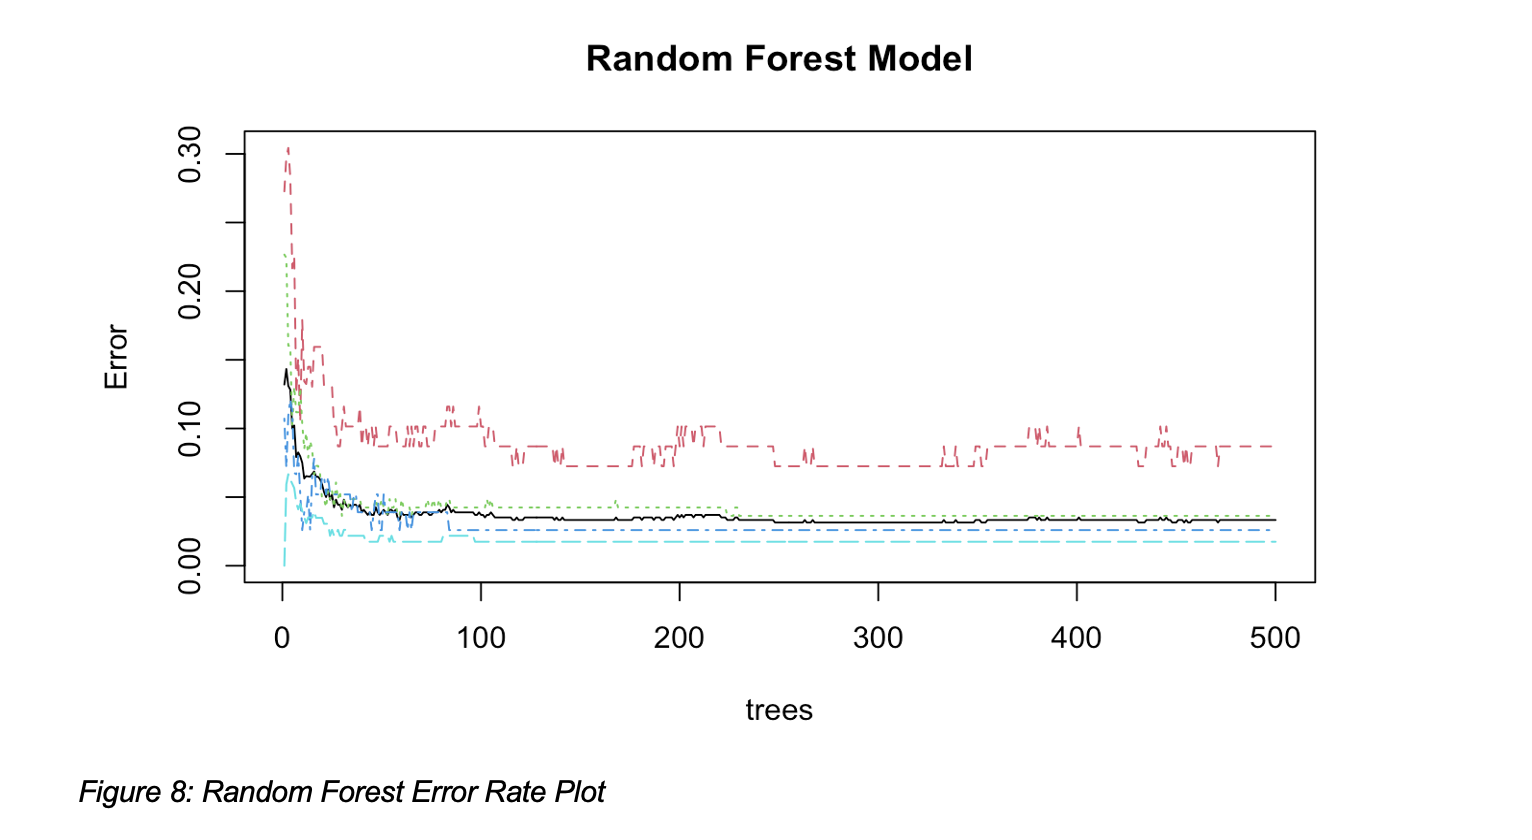
\includegraphics[width = \linewidth]{Figure/figure8.png}
    \label{fig:enter-label}
\end{figure}
\begin{figure}[ht]
    \centering
    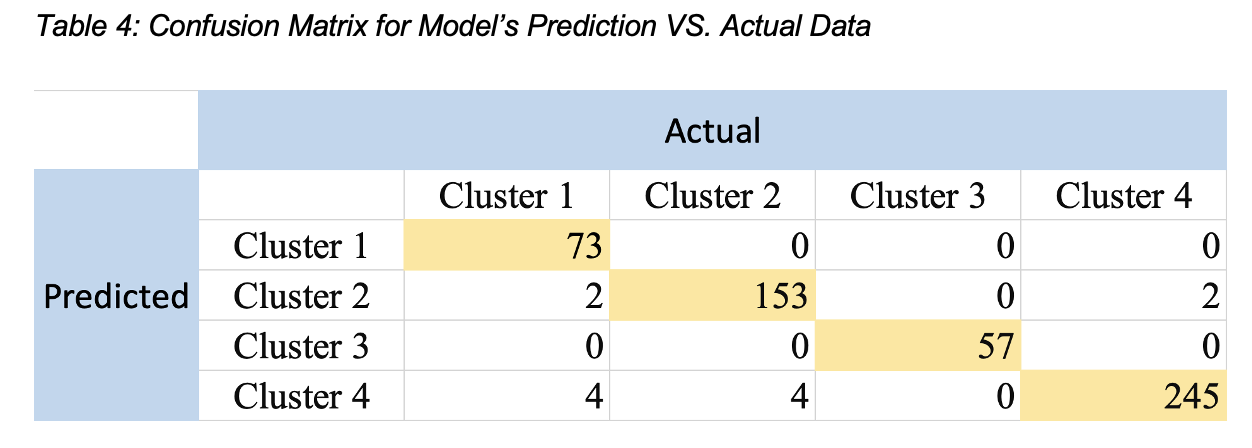
\includegraphics[width = \linewidth]{Figure/table4.png}
    \label{fig:enter-label}
\end{figure}
\\The confusion matrix (Table 4) further reflects the model's practical effectiveness, with a 97.78\% prediction accuracy,  in distinguishing between players of different performance levels. However, some confusion between closely rated classes suggests areas for refinement, perhaps by incorporating more granular data or tweaking model parameters.\\
In conclusion, this Random Forest model effectively harnesses the inherent randomness and collective decision-making power of multiple trees to yield highly accurate predictions. Its ability to identify and utilize key performance indicators, combined with its robust error handling, renders it a valuable tool for analyzing NBA player performance, offering reliable insights crucial for team management strategies, player evaluations, and game-day decisions.
\section*{Discussion and Conclusion}
\addcontentsline{toc}{section}{Discussion and Conclusion}
The findings of this study provide valuable insights into the diverse roles and performance profiles of NBA players. By combining dimensionality reduction, clustering, and ensemble learning techniques, the analysis effectively segments players into distinct clusters that reflect their strengths, specializations, and contributions to the game.\\
The Consistent Role Players cluster represents reliable contributors who excel in specific roles, often as secondary scorers or defensive anchors. The Developing Perimeter Players cluster captures players transitioning into more central roles, leveraging their proficiency in perimeter shooting and outside scoring. The All-Stars cluster comprises the league's elite performers, showcasing versatility in scoring from various ranges, playmaking abilities, and leadership on the court. Finally, The Supportive Contributors cluster highlights players who may not be primary scorers but contribute through situational plays, defensive efforts, and maintaining team dynamics.\\
The Random Forest model's emphasis on Offensive Rebounds, Field Goals, Blocks, and Points as key performance indicators underscores the importance of scoring efficiency, defensive impact, and offensive rebounding in determining player value. These findings align with modern basketball trends that prioritize versatility, spacing, and efficient scoring from multiple areas of the court.\\
The study's insights can inform team-building strategies, player evaluation, and roster construction decisions. By identifying the strengths and specializations of different player archetypes, teams can optimize their lineups, allocate roles effectively, and foster synergistic on-court dynamics. Additionally, the analysis can guide player development efforts, highlighting areas for improvement and potential avenues for growth.\\
Future research could explore the integration of advanced metrics, such as player tracking data and shot quality analysis, to further refine the player classification and performance prediction models. Incorporating team-level statistics and lineup data could also provide insights into optimal team compositions and player synergies.\\
While this study provides valuable insights into predicting NBA player performance using clustering and random forest techniques, it is important to acknowledge its limitations. One notable limitation is the reliance on data from a single NBA season. By focusing on a specific season, the model's predictive power may be influenced by the unique characteristics, trends, and dynamics of that particular year. Player performance can vary from season to season due to factors such as team changes, injuries, player development, and strategic adjustments. Therefore, the findings of this study may not be fully generalizable to other NBA seasons or future player performances. To address this limitation, future research could expand the scope of the analysis by incorporating data from multiple NBA seasons. By training the model on a more comprehensive dataset spanning several years, the predictive capabilities of the random forest model could be enhanced, capturing a wider range of player performances and accounting for season-to-season variations. This approach would provide a more robust and reliable assessment of the model's ability to predict player cluster membership and performance across different contexts.\\
Additionally, incorporating data from multiple seasons would allow for the exploration of player development trajectories and the identification of patterns or trends that emerge over time. This longitudinal perspective could offer valuable insights into how players evolve and transition between clusters throughout their careers, enabling a more dynamic understanding of player performance and potential.\\
To conclude, this study demonstrates the power of data-driven analysis in understanding and assessing NBA player performances, offering a comprehensive framework for evaluating talent and informing strategic decision-making within the dynamic landscape of professional basketball.
\newpage
\begin{thebibliography}{99}

\bibitem{Dehesa2019}
R.~Dehesa, A.~Vaquera, B.~Gonçalves, N.~Mateus, M.~Á.~Gomez-Ruano, and J.~Sampaio,
\textit{Key Game Indicators in NBA Players’ Performance Profiles},
Kinesiology, vol. 51, 2019. https://doi.org/10.26582/k.51.1.9

\bibitem{Nguyen2021}
N.~H.~Nguyen, D.~T.~A.~Nguyen, B.~Ma, and J.~Hu,
\textit{The Application of Machine Learning and Deep Learning in Sport: Predicting NBA Players’ Performance and Popularity},
Journal of Information and Telecommunication, vol. 6, Informa UK Limited, 2021. https://doi.org/10.1080/24751839.2021.1977066

\bibitem{ZhangGTP}
S.~Zhang, A.~Lorenzo, M.-A.~Gómez, H.~Liu, B.~Gonçalves, and J.~Sampaio,
\textit{Players’ Technical and Physical Performance Profiles and Game-to-Game Variation in NBA}, 2017.

\bibitem{NainChi}
Y.~Nain and J.~Chi,
\textit{A Mixed Model for Performance-Based Classification of NBA Players}, n.d.

\bibitem{ZhangCP}
S.~Zhang, A.~Lorenzo, M.-A.~Gómez, N.~Mateus, B.~Gonçalves, and J.~Sampaio,
\textit{Clustering Performances in the NBA According to Players’ Anthropometric Attributes and Playing Experience}, 2018.

\end{thebibliography}
\end{document}